% Unofficial Yale Poster template (forks listed in the original header).

\documentclass[final]{beamer}

% ====================
% Packages
% ====================

\usepackage[T1]{fontenc}
\usepackage[utf8]{luainputenc}
\usepackage{lmodern}
\usepackage[size=custom, width=122,height=91, scale=1.05]{beamerposter}
\usetheme{gemini}
\usecolortheme{msu}
\usepackage{graphicx}
\usepackage{booktabs}
\usepackage{array}
\usepackage{tikz}
\usetikzlibrary{positioning}
\usepackage{pgfplots}
\pgfplotsset{compat=1.14}
\usepackage{anyfontsize}

% ====================
% Lengths
% ====================

% If you have N columns, choose \sepwidth and \colwidth such that
% (N+1)*\sepwidth + N*\colwidth = \paperwidth
\newlength{\sepwidth}
\newlength{\colwidth}
\setlength{\sepwidth}{0.025\paperwidth}
\setlength{\colwidth}{0.3\paperwidth}

\newcommand{\separatorcolumn}{\begin{column}{\sepwidth}\end{column}}

% ====================
% Title
% ====================

\title{KernelForge: Measured LLM-Generated Triton Kernels}

% List ALL team members, comma-separated. Use the order agreed inside the team.
\author[KernelForge Team]{Imanol Armando González Solís, José Manuel Martínez Morales, Pablo Esteban Reyes Herrera\texorpdfstring{\\[-0.2ex]}{, }
Sebastian Gerritsen Ortiz, Victor Javier Quintana Cisneros}

\institute[shortinst]{Tecnológico de Monterrey — TC3002B (ACA-2026)}

% ====================
% Footer (optional)
% ====================

\footercontent{
  \href{https://github.com/JoseMartinezM/KernelForge}{github.com/JoseMartinezM/KernelForge} \hfill
  TC3002B — ACA-2026 \hfill
  \href{mailto:kernelforge-team@tec.mx}{kernelforge-team@tec.mx}}

% ====================
% Logo (optional)
% ====================

% Left: institution logo (Tec de Monterrey)
\IfFileExists{logos/logo.png}{\logoright{
\includegraphics[height=6.5cm]{logos/logo.png}}}{}
% Right: partner / funding agency logo (uncomment when available)
%\logoright{\includegraphics[height=7cm]{logos/partner.png}}

% ====================
% Body
% ====================

\begin{document}

\begin{frame}[t]
\begin{columns}[t]
\separatorcolumn

% ============================================================
% COLUMN 1 — Motivation, problem, related work
% ============================================================
\begin{column}{\colwidth}

  \begin{block}{Abstract}

    KernelForge studies when LLM-generated Triton GPU kernels are worth writing,
    and whether grammar/planner interventions improve over plain Gemma 4 code
    generation. The project combines TritonBench-T~[1] prompt and ledger tooling,
    grammar-constrained decoding, a lightweight semantic checker, and KAGBench:
    our project-created benchmark adapter for agentic kernel workflows. The measured result is deliberately
    mixed: generated Triton kernels can be much faster than PyTorch references on
    favorable memory-bound and fusion-friendly operators, with a verified
    11.25\(\times\) KAGBench speedup, but our constrained/planner variants do not
    show a statistically reliable correctness improvement over no-grammar or
    plain Gemma 4 baselines. The reusable artifact is the evidence loop: prompts,
    candidates, repairs, correctness, timing, and caveats are all preserved as
    JSONL traces for later fine-tuning or preference-data experiments.

  \end{block}

  \begin{block}{1. Problem statement}

    \begin{itemize}
      \item \textbf{Pain point:} GPU researchers and library authors spend repeated effort turning tensor math into correct, masked, launchable Triton kernels.
      \item \textbf{Current baseline:} Raw LLM completions often look plausible but fail through bad APIs, missing masks, wrapper mismatches, or numerical errors.
      \item \textbf{Our research question:} Can grammar constraints or planner--implementer decomposition improve over plain Gemma 4, and which generated kernels actually beat PyTorch?
    \end{itemize}

  \end{block}

  \begin{block}{2. Background}

    A context-free grammar describes which token sequences belong to a language.
    For Triton, grammar rules are a practical middle layer: stricter than natural
    language prompting, but lighter than a full compiler. XGrammar uses those
    rules during decoding so the model is guided toward legal Triton JIT blocks.
    Triton~[2] is a good target because it exposes GPU programming through Python-like
    kernels while still compiling to efficient device code.

    \begin{itemize}
      \item \textbf{Formal grammars:} BNF/GBNF rules define the allowed shape of Triton JIT functions.
      \item \textbf{Constrained decoding:} The model is restricted to grammar-valid continuations while generating code.
      \item \textbf{Triton DSL:} A Python-embedded language for writing GPU kernels with explicit blocks, masks, and program IDs.
    \end{itemize}

  \end{block}

  \begin{alertblock}{3. Our differentiator}

    \textbf{One-line differentiator:} KernelForge is a measured generation loop,
    not only a demo generator: it tests plain Gemma 4 against constrained and
    planner--implementer variants, then keeps reusable traces for future tuning
    even when the measured answer is \emph{no correctness improvement}.

    \begin{itemize}
      \item \textbf{C1.} The planner emits explicit sections for pattern, API contract, program mapping, numerics, non-default choices, and risks before code is written.
      \item \textbf{C2.} The implementer receives the plan plus hard Triton rules, optional grammar constraints, and public-test context.
      \item \textbf{C3.} Plans, candidates, failures, repair directives, paired correctness, and speed measurements form a base for future fine-tuning, distillation, or preference ranking.
    \end{itemize}

  \end{alertblock}

\end{column}

\separatorcolumn

% ============================================================
% COLUMN 2 — Methodology, grammar design, pipeline
% ============================================================
\begin{column}{\colwidth}

  \begin{block}{4. System architecture}

    \begin{figure}
      \centering
      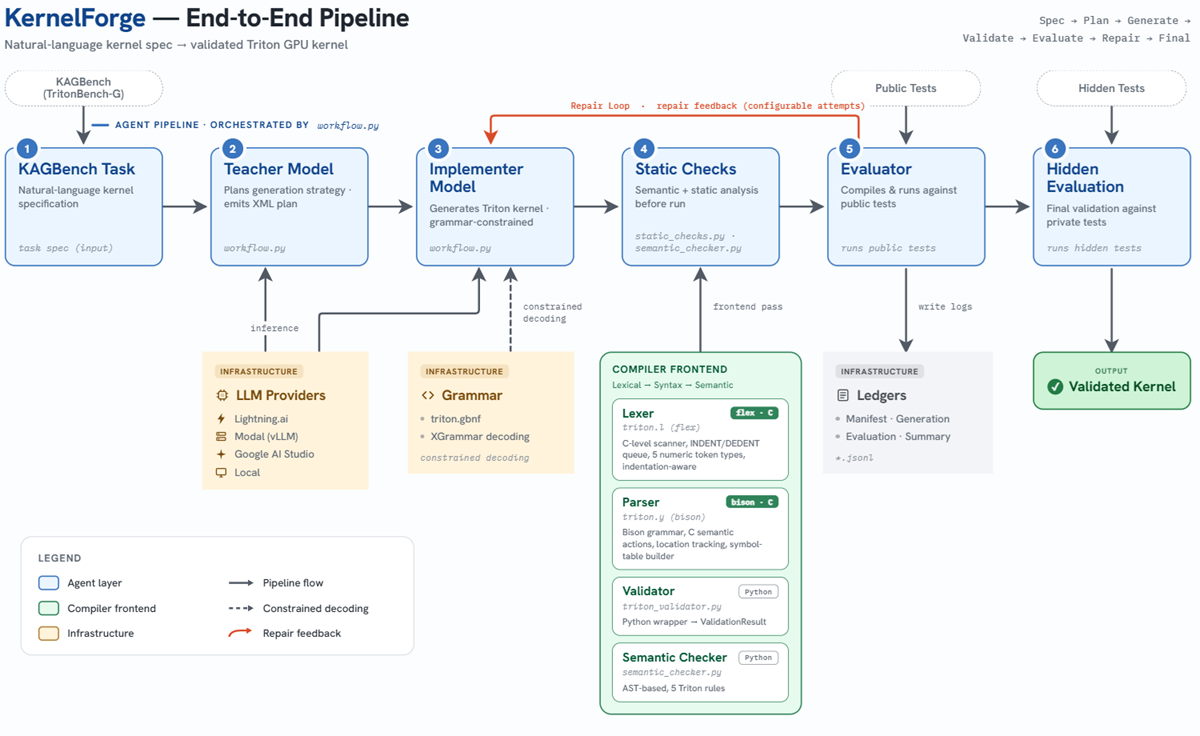
\includegraphics[width=0.88\linewidth]{figures/architecture.png}
      \caption{KernelForge end-to-end pipeline: from kernel specification to checked candidate, GPU evaluation, repair feedback, and reusable ledgers.}
    \end{figure}

    KAGBench (Kernel Agentic Bench) is a 48-task dataset created inside this
    project to make TritonBench-derived cases fit an agentic loop. Each case is a
    self-contained folder with a prompt, PyTorch reference, public tests, hidden
    tests, tags, and source provenance. A teacher/planner writes a compact
    strategy; an implementer emits a Triton candidate; static checks, GPU
    evaluation, optional repair prompts, and JSONL ledgers preserve the full
    trace for benchmarking and later training data.

  \end{block}

  \begin{block}{5. Grammar design}

    \begin{itemize}
      \item \textbf{L1 — Skeleton:} \texttt{@triton.jit} decorators, Python function headers, parameters, and bounded indentation.
      \item \textbf{L2 — Declarations:} annotated/default parameters, including \texttt{BLOCK\_SIZE: tl.constexpr} and local assignments.
      \item \textbf{L3 — Expressions:} arithmetic, comparisons, tuple/list expressions, indexing, and qualified calls such as \texttt{tl.load}.
      \item \textbf{L4 — Control flow:} bounded \texttt{if}, \texttt{for}, \texttt{while}, and \texttt{with} blocks inside Triton JIT bodies.
    \end{itemize}

    The grammar intentionally focuses on Triton JIT blocks instead of arbitrary
    Python modules. Imports, benchmark wrappers, and test harness code stay
    outside the constrained region because the benchmark adapters need flexible
    signatures and glue code. The active artifact is
    \texttt{grammar/triton.gbnf}; current tests smoke-compile it through XGrammar
    and check representative accept/reject snippets. It is still an experiment,
    not a complete Triton parser.

  \end{block}

  \begin{block}{6. Generation pipeline}

    \begin{enumerate}
      \item \textbf{Prompt construction:} Build a prompt from a KAGBench case derived from TritonBench-T, including the task description, expected wrapper behavior, PyTorch reference, and optional public tests.
      \item \textbf{Planner stage:} Ask a planning model for the kernel pattern, API contract, program mapping, numerics, and likely risks without writing code.
      \item \textbf{Implementer stage:} Generate code from the plan at temperature 0; when enabled, pass \texttt{grammar/triton.gbnf} to vLLM with the \texttt{xgrammar} backend.
      \item \textbf{Static triage:} Reject empty or unparsable outputs for evaluation, and log semantic warnings for missing masks, decorators, program IDs, or suspicious PyTorch calls.
      \item \textbf{Compile \& run:} Evaluate generated code against public or hidden tests with a local subprocess or Modal GPU backend.
      \item \textbf{Repair/data loop:} When public evaluation fails, feed the error summary back to the planner/implementer loop and preserve every attempt as data for analysis or future tuning.
    \end{enumerate}

  \end{block}

\end{column}

\separatorcolumn

% ============================================================
% COLUMN 3 — Experimental setup, results, conclusions, references
% ============================================================
\begin{column}{\colwidth}

  \begin{exampleblock}{7. Experimental setup}

      \begin{itemize}
      \item \textbf{Benchmark data:} TritonBench-T simple set (166 tasks) for raw/LLGuidance baselines; KAGBench, our 48-task project-created adapter from TritonBench-G/T cases, for planner--implementer and repair experiments.
      \item \textbf{Hardware:} Modal L4 for the Gemma 4 vLLM backend; local ROCm/Triton subprocesses for KAGBench candidate evaluation and timing.
      \item \textbf{Software:} Python/uv workflow, PyTorch + Triton evaluation environment, vLLM structured outputs, llama.cpp/LLGuidance GBNF constraints, and JSONL ledgers.
      \item \textbf{Repetitions:} Correctness-first evaluation per candidate; speed timing on hidden-passing candidates with \texttt{triton.testing.do\_bench}. Top KAGBench speedups were retested with warmup=100, rep=1000, 5 repeats.
      \item \textbf{Metrics/data:} call@1, exe@1, public/hidden pass, mismatch summaries, semantic warnings, truncation, latency, planner text, candidate code, repair traces, and speedup over PyTorch references.
    \end{itemize}

  \end{exampleblock}

  \begin{block}{8. Results}

    \textbf{Headline result:} generated Triton can be \textbf{11.25\(\times\)}
    faster than the PyTorch reference on a favorable KAGBench embedding task, but
    \textbf{our completed paired comparisons show no reliable correctness gain
    from constraints or planning}. That negative result is part of the evidence:
    the ledgers let us separate real speedups from generation-method claims.

    \begin{table}
      \centering
      \scriptsize
      \setlength{\tabcolsep}{3pt}
      \begin{tabular}{@{}>{\raggedright\arraybackslash}p{0.25\linewidth} >{\raggedright\arraybackslash}p{0.15\linewidth} >{\raggedright\arraybackslash}p{0.25\linewidth} >{\centering\arraybackslash}p{0.10\linewidth} >{\raggedright\arraybackslash}p{0.13\linewidth}@{}}
        \toprule
        \textbf{Method} & \textbf{Scope} & \textbf{Pass rate} & \textbf{Median} & \textbf{Paired result} \\
        \midrule
        Plain Gemma 4 vLLM, no grammar & TritonBench-T (166) & call@1 40/166; exe@1 21/166 & 1.01\(\times\) & Baseline \\
        Gemma 4 + LLGuidance/GBNF & TritonBench-T (166) & call@1 32/166; exe@1 21/166 & 1.00\(\times\) & exe@1 tie; \(p=1.000\) \\
        Planner + GBNF constrained & KAGBench (48) & public 25/48; hidden 16/48 & 1.10\(\times\) & no gain; \(p=1.000\) \\
        Planner, no grammar & KAGBench (48) & public 22/48; hidden 17/48 & 1.09\(\times\) & KAGBench baseline \\
        \bottomrule
      \end{tabular}
      \caption{Completed runs show no statistically reliable correctness gain from constraints or planner--implementer decomposition, while correctness-passing Triton kernels can still provide real speedups over PyTorch references.}
    \end{table}

    \begin{figure}
      \centering
      \begin{tikzpicture}
        \begin{axis}[
          xbar,
          xmin=0,
          xmax=12,
          xtick={0,3,6,9,12},
          minor x tick num=0,
          width=0.92\linewidth,
          height=6.6cm,
          xlabel={Verified speedup over PyTorch reference},
          symbolic y coords={dropout,dequant,l2,embedding},
          ytick=data,
          yticklabels={dropout,dequantize,L2 norm,embedding},
          nodes near coords={\pgfmathprintnumber[fixed,precision=2]{\pgfplotspointmeta}\(\times\)},
          point meta=x,
          every node near coord/.append style={font=\scriptsize},
          axis x line*=bottom,
          axis y line*=left,
          enlarge y limits=0.2,
        ]
          \addplot+[fill=blue!70] coordinates {
            (2.39,dropout)
            (2.62,dequant)
            (3.26,l2)
            (11.25,embedding)
          };
        \end{axis}
      \end{tikzpicture}
      \caption{How generated kernels produced speedup: the best candidates used direct Triton program mapping, masked block loads/stores, in-kernel reductions or simple fused arithmetic, and avoided PyTorch dispatch/intermediate tensors. These wins are operator-dependent; matrix-multiply-like cases often lose to vendor libraries.}
    \end{figure}

  \end{block}

  \begin{block}{9. Contributions \& limitations}

    \begin{itemize}
      \item \textbf{Reusable contribution:} KAGBench plus the ledgers provide a base for an agentic improvement loop: passing kernels become supervised examples, failed repairs become edit data, and multiple candidates can become preference/ranking data.
      \item \textbf{Main Triton advantage:} Memory-bound or fusion-friendly tasks can use one custom kernel to avoid PyTorch dispatch, intermediate tensors, and implicit dtype/masking choices.
      \item \textbf{What changed over plain Gemma 4?} Not correctness so far: LLGuidance tied plain Gemma 4 on TritonBench-T exe@1, and KAGBench constrained/no-grammar hidden-pass differences were not significant.
      \item \textbf{How models generated speedup:} Winning candidates used one-program-per-row/block mappings, \texttt{tl.arange} offsets, masked \texttt{tl.load}/\texttt{tl.store}, in-kernel reductions, and fused elementwise arithmetic.
      \item \textbf{Caveats:} Local LLGuidance was slower than Modal vLLM plain Gemma 4, complete KAGBench constraints used llama.cpp GBNF, and speedups are measured only on correctness-passing candidates.
    \end{itemize}

  \end{block}

  \begin{block}{References}

    \scriptsize
    \setlength{\parindent}{0pt}
    \setlength{\parskip}{0.25em}
    \hangindent=1.7em\hangafter=1
    [1] J. Li \emph{et al.}, ``TritonBench: Benchmarking large language model capabilities for generating Triton operators,'' in \emph{Findings of ACL}, 2025, pp. 23053--23066, doi: 10.18653/v1/2025.findings-acl.1183.

    \vspace{0.25em}
    \hangindent=1.7em\hangafter=1
    [2] P. Tillet, H. T. Kung, and D. Cox, ``Triton: An intermediate language and compiler for tiled neural network computations,'' in \emph{Proc. MAPL}, 2019, pp. 10--19, doi: 10.1145/3315508.3329973.

  \end{block}

\end{column}

\separatorcolumn
\end{columns}
\end{frame}

\end{document}
